\documentclass[11pt,a4paper]{scrartcl}
\usepackage[utf8]{inputenc}
\usepackage[italian]{babel}

\usepackage{amsmath, amsfonts, amssymb}
\usepackage{graphicx, booktabs}

\usepackage{parskip}

\author{L. De Sano, A. Donizetti, M. Scotti}
\title{Risoluzione di sistemi lineari sparsi \\con Python e Scipy}
\date{Maggio 2014}


\begin{document}
\maketitle
\begin{abstract}
Descriviamo l'utilizzo del linguaggio Python e di un ambiente di librerie denominato \emph{Scipy} per la risoluzione di sistemi lineari sparsi.
\end{abstract}

\section*{Python e Scipy}

In questa sezione diamo una descrizione del linguaggio di programmazione (Python) e dell'ambiente di librerie per il calcolo scientifico (Scipy) utilizzati nel progetto. Dettagliamo i criteri che hanno orientato la scelta, e spieghiamo brevemente come e perché Python e Scipy soddisfano effettivamente le nostre aspettative.

\subsection*{Python}

Python\footnote{\texttt{python.org}} è un linguaggio di programmazione \emph{open-source}, \emph{general-purpose} e di alto livello che supporta vari paradigmi di programmazione (tra cui imperativo, ad oggetti, funzionale). È un linguaggio dinamico con una sintassi che facilita la scrittura di codice mantenibile e leggibile, ed è considerato particolarmente adatto per lo sviluppo rapido di applicazioni software e/o di scripting. Poiché tutti e tre i componenti del gruppo avevano esperienza pregressa di programmazione in Python, l'abbiamo immediatamente preso in considerazione.

Le caratteristiche da noi desiderate per l'ambiente con cui effettuare l'esecuzione dei test proposti sui sistemi lineari sparsi sono le seguenti:
\begin{itemize}
	\item \textbf{rapidità di sviluppo}: il linguaggio deve permettere lo sviluppo rapido di codice anche poco strutturato (in totale qualche centinaio di righe di codice che effettuano il setup delle librerie ed eseguono una serie di test);
	\item \textbf{maturità del linguaggio}: il linguaggio deve essere diffuso, ben supportato su varie piattaforme di computazione, semplice da installare e ben documentato;
	\item \textbf{disponibilità di librerie}: il linguaggio deve essere dotato di una libreria per il calcolo scientifico (e in particolar modo per la manipolazione di matrici sparse) ben testata e ben documentata (sia a livello di documentazione primaria, sia per quanto riguarda la disponibilità di materiale esterno come tutorial e discussioni riguardo problemi e modalità d'utilizzo della libreria stessa);
	\item \textbf{performances}: il linguaggio (e le sue librerie) devono fornire gli strumenti adatti ad eseguire computazioni di natura pesantamente numerica in maniera efficiente (ovvero il linguaggio di per sé non deve astrarre troppo dall'architettura hardware del calcolatore, o qualora lo faccia deve fornire un'interfaccia che consenta la chiamata di procedure di basso livello, ad esempio scritte in altri linguaggi di programmazione);
\end{itemize}

Il requisito sulla rapidità di sviluppo è stato il principale motivo per cui abbiamo deciso di escludere in prima battuta l'utilizzo di alcuni dei linguaggi compilati tipicamente usati in ambito computazione scientifica (C, C++, FORTRAN), e di orientarci sulla categoria dei linguaggi dinamici (in genere molto più versatili e adatti all'ambito scripting e software prototyping). 

Per quanto riguarda la maturità dell'ambiente di programmazione, è indubbio che il Python soddisfi il requisito sopracitato: il linguaggio è diffusamente utilizzato, ben documentato, ben supportato e attivamente sviluppato. Decisamente ben pubblicizzata è anche l'esistenza di un ambiente di programmazione adatto alla computazione scientifica (Scipy), su cui ci soffermeremo nella sezione successiva. L'interprete originale (CPython) e le librerie standard sono preinstallati sulla maggior parte dei sistemi Linux e su OS X, ed è disponibile un installer per i sistemi Windows. L'installazione di librerie aggiuntive (distribuite separatamente da quella standard) è lievemente più complicata, soprattutto nel caso di codice che ha anche dipendenze esterne (come nel caso di Scipy).

L'ultimo punto è l'unico che avrebbe potuto rivelarsi problematico: è noto come i linguaggi dinamici (solitamente interpretati, come appunto lo è il Python) tipicamente hanno la peggio nel confronto con i linguaggi compilati in termini di \emph{performances}\footnote{Questo è ancora più evidente per codice dinamico sviluppato rapidamente e senza che la questione performances sia stata considerata accuratamente durante lo fase di progettazione}. Per questo motivo, nella scelta delle librerie esterne da utilizzarsi per la manipolazione di matrici, abbiamo avuto cura di utilizzare un ambiente di programmazione (Scipy, appunto) che non fosse completamente scritto in Python puro, ma che mettesse invece a disposizione un'interfaccia Python per l'utilizzo di librerie \emph{high-performances} scritte in altri linguaggi, e opportunamente racchiuse in \emph{wrappers} Python. Questo ci ha consentito di utilizzare a nostro vantaggio la rapidità di sviluppo fornita da un linguaggio dinamico senza tuttavia dover rinunciare ad ottenere ottime \emph{performaces} sulle computazioni numeriche effettuate durante i test.


\subsection*{Scipy}
Scipy\footnote{\texttt{scipy.org}} è un ecosistema di librerie \emph{open-source} pensate per la scrittura di codice nell'ambito della computazione scientifica. Consiste in una serie di pacchetti (strettamente integrati tra loro) che implementano funzionalità di manipolazione array multidimensionali (Numpy), calcolo numerico ed ottimizzazione (Scipy-library), realizzazione di grafici e schemi (Matplotlib) e computazioni simboliche (Sympy).

Come anticipato nella sezione precedente, per eseguire computazioni numericamente intensive scritte in Python a livelli di \emph{performances} accettabili è necessario delegare la maggior parte delle operazioni di basso livello a librerie specializzate, sviluppate in linguaggi più adatti a tale compito. Scipy non fa eccezione e, pur mantenendo un'interfaccia di alto livello, esegue buona parte delle computazioni numeriche affidandosi a del codice che gira al di fuori dell'interprete Python e scritto in \texttt{C} o in \texttt{FORTRAN}. 

Per quanto riguarda lo stato di salute della libreria, Scipy è attualmente attivamente sviluppato. Come è possibile apprendere da sito ufficiale del progetto, l'ultimo rilascio di Scipy e Numpy è del 3 maggio 2014. Tutto lo sviluppo delle librerie è effettuato su Github, e questo permette una grande flessibilità di sviluppo: centinaia di sviluppatori sottomettono al gruppo di lavoro i propri miglioramenti, e il progetto di cresce rapidamente acquisendo funzionalità sempre nuove. Peraltro, come succede per ogni altro software, e soprattutto per quelli opensource, nelle librerie sono presenti alcuni bug, e alcune funzionalità dei pacchetti sono attualmente prototipate ma non ancora implementate.

La sezione dove sono discusse tematiche relative all'utilizzo del progetto è molto ricca, ed è estremamente facile trovare in rete tutorial scritti da terze parte e risposte ad eventuali problemi incontrati durante lo sviluppo del codice. In caso di segnalazione di bug e/o difetti, la comunity è molto attenta e rapida nel dare una risposta alla questione posta. 

% non ho capito bene che vuol dire:
% --> "Tutte le librerie che compongono l'ambiente Scipy  hanno una milestone molto ricca"  <--
%
% che prevede l'introduzione di sempre nuove funzionalità di analisi e simulazione oltre al miglioramento e alla risoluzione delle problematiche aperte.
%
% TODO: de-commentare il paragrafo una volta chiarita la questione

\subsection*{Scipy per la soluzione di sistemi sparsi}

Per la risoluzione dei sistemi lineari sparsi abbiamo utilizzato il modulo \texttt{scipy.sparse} (per l'importazione e la manipolazione di matrici sparse) e il sottomodulo \texttt{scipy.sparse.linalg} (che contiene i risolutori diretti e iterativi specializzati per operare su matrici sparse). Entrambi i moduli utilizzano a loro volta il pacchetto \texttt{numpy}.

Per la manipolazione di matrici, \texttt{numpy} utilizza prevalentemente codice C e chiamate a ATLAS\footnote{Implementazione \emph{open-source} di BLAS} e LAPACK\footnote{Linear Algebra PACKage, scritto in FORTRAN}, mentre il modulo \texttt{scipy.sparse.linalg} utilizza UMFPACK\footnote{Unsymmetric multifrontal sparse LU factorization package (\texttt{cise.ufl.edu/research/sparse/umfpack}), scritto in C e chiamato tra l'altro dall'operatore $\setminus$ di Matlab quando le matrici sono sparse} e SuperLU\footnote{Supernodal LU (\texttt{crd-legacy.lbl.gov/$\sim$xiaoye/SuperLU})} per i risolutori diretti. I risolutori iterativi sono implementati in Python puro, ma possono venire precondizionati tramite fattorizzazioni LU parziali calcolate da SuperLU, e risultano quindi in ogni caso abbastanza veloci.

Proprio a causa di queste dipendenze esterne, l'installazione di Scipy è maggiormente soggetta a problemi rispetto a quanto accade solitamente con altre librerie Python. Nonostante l'ambiente Scipy sia ben strutturato a livello di pacchetti e supportato, la modalità di installazione più semplice prevede l'utilizzo almeno di un \emph{package-manager} di sistema (tipicamente presenti su sistemi Linux, vedi aptitude), che si occupa anche di installare e linkare pacchetti esterni (implementazioni BLAS, UMFPACK e altri). La presenza di queste librerie è fondamentale per il funzionamento di Scipy, e non è del tutto banale configurare correttamente il sistema per usarle nel caso si scelga di effettuare un'installazione manuale.

Le dipendenze esterne vanno anche a compromettere leggermente la portabilità del linguaggio: se è quasi garantito che del codice che utilizza solamente la libreria standard sia in grado di girare su sistemi diversi, abbiamo riscontrato invece delle inconsistenze (sulle quali dettaglieremo in seguito) nell'esecuzione su calcolatori differenti di test che utilizzano codice Scipy. 


\section*{Risoluzione di sistemi sparsi}

In questa sezione diamo una descrizione della progettazione, della scrittura e dell'esecuzione dei test proposti. Il lavoro si è svolto sostanzialmente in due fasi: in prima battuta è stato affrontato il problema di leggere le matrici dai files e memorizzare le stesse in RAM in un formato opportuno, successivamente è stato sviluppato il codice che si occupa di chiamare i vari risolutori messi a disposizione da Scipy, misurare tempi di esecuzione ed errori sui risultati, e infine esportare i risultati.

\subsection*{Lettura dei file e memorizzazione}
Date le dimensioni complessive dei files contenenti le matrici (circa 290 MB), una prima questione da affrontare riguarda la scelta di una modalità di lettura e costruzione delle strutture dati che sia il più efficiente possibile. In particolare, è desiderabile ottimizzare i tempi di lettura dal disco, lo spazio occupato dalle matrici in RAM, e i tempi di esecuzione dei metodi per la risoluzione dei sistemi lineari sparsi che esse rappresentano.

Per la lettura da disco ci sono (almeno) tre modi di operare:
\begin{itemize}
\item \textbf{Handmade, non bufferizzato}: scrivere uno script Python che legge i dati dal disco, senza bufferizzazione, e costruisce in maniera incrementale le matrici sparse
\item \textbf{Handmade, bufferizzato}: uno script Python che legge i dati dal disco, con bufferizzazione (ovvero lettura di grossi blocchi di dati e costruzione per blocchi)
\item \textbf{mmread}: un metodo messo a disposizione da \texttt{scipy.io} per la lettura di matrici memorizzate in formato Matrix Market\footnote{\texttt{math.nist.gov/MatrixMarket/formats.html\#MMformat}}
\end{itemize}

Il primo (handmade, non bufferizzato) è certamente il più ingenuo. Non è stato realmente preso in considerazione in fase di scrittura del codice, ma ne abbiamo implementato una versione di prova per verificare quanto effettivamente possa costare, in termini di tempi di esecuzione, uno script di importazione dati che sia stato progettato sbadatamente. Il secondo (handmade, bufferizzato) garantisce una buona velocità di lettura e ci ha consentito di utilizzare direttamente i file forniti. Il terzo (\texttt{mmread}) è il più performante, e sicuramente quello che richiede meno lavoro nel caso i file siano formattati secondo lo standard Matrix Market.

\begin{figure}[!ht]
\centering
\begin{tabular}{l|cc}
\toprule
& time & speed \\
\midrule
nonbuff & 121.56 secs & 1.56 MB/s \\
buff & 27.38 secs & 6.92 MB/S \\
\texttt{mmread} & 12.34 secs & 15.62 MB/s \\
\bottomrule
\end{tabular}
\end{figure}

\begin{figure}[!ht]
\centering
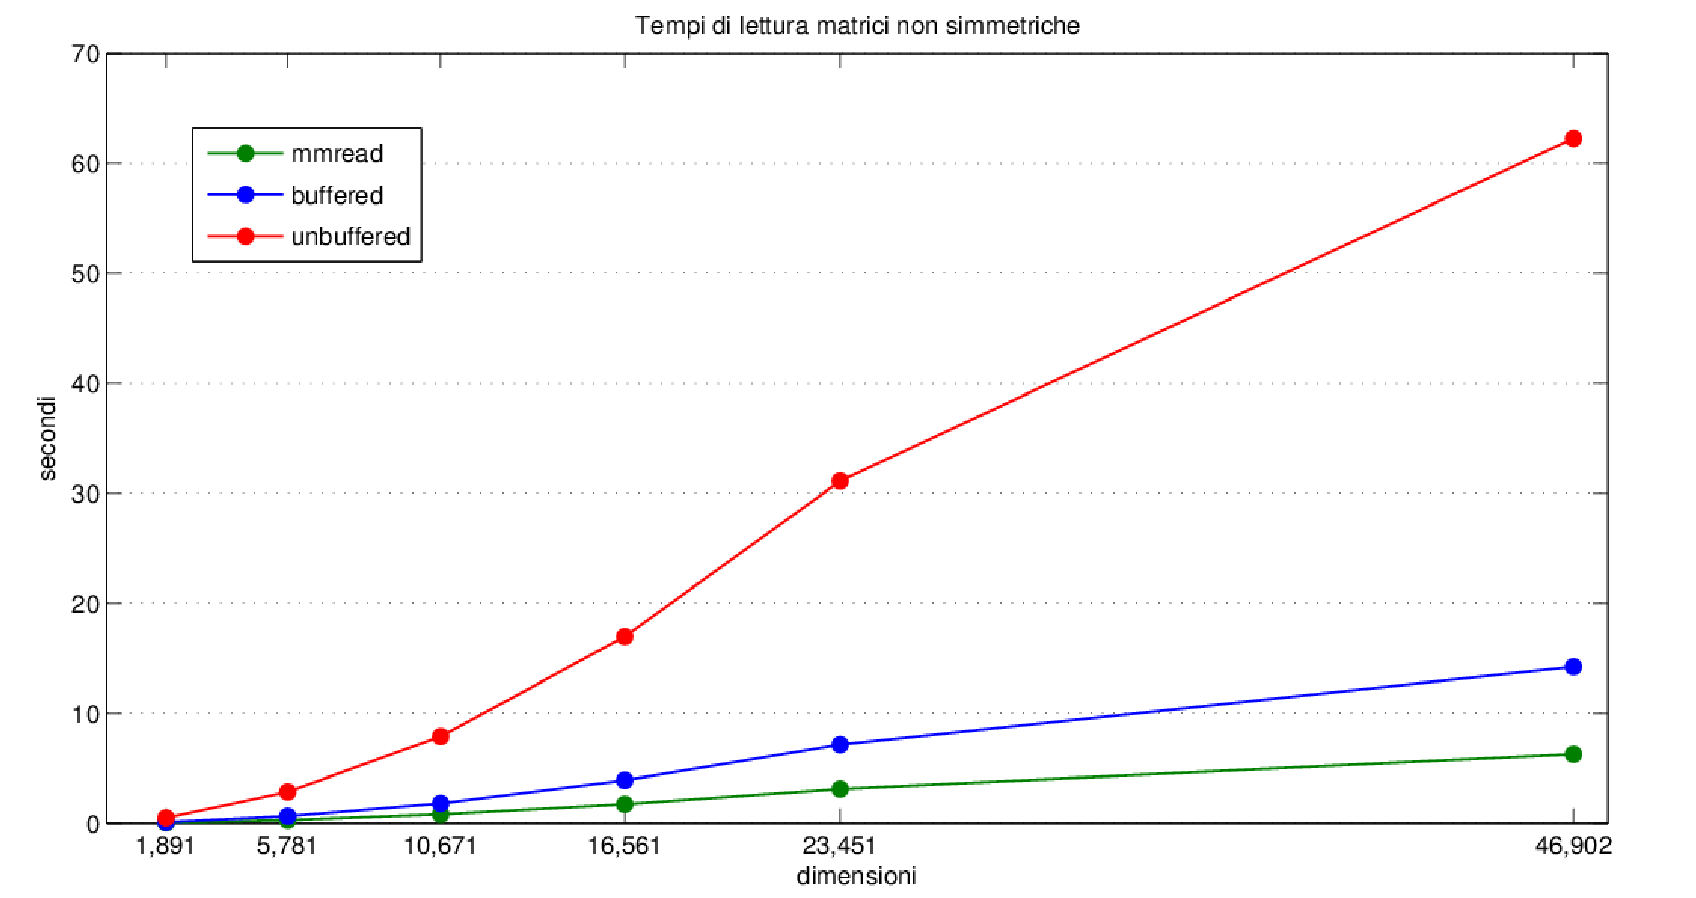
\includegraphics[scale=0.52]{images/lettura} 
\end{figure}

In grafico sono riportati i risultati di tre test di lettura eseguiti sulle sei matrici non simmetriche. Come si può vedere, uno script che sia ben progettato (e che bufferizzi le letture) è equiparabile in velocità di lettura al metodo \texttt{mmread} fornito da \texttt{scipy}, mentre uno non particolarmente ben scritto scala decisamente male rispetto all'aumentare delle dimensioni dei files.

In fase di test dei metodi risolutivi abbiamo infine optato per l'utilizzo di \texttt{mmread} (il più rapido), dopo aver convertito le matrici scaricate nel formato Matrix Market e averne salvato i file.

\subsection*{Metodi diretti}
% metodi disponibile
% tempi di esecuzione
% errori sulla soluzione

\subsection*{Metodi iterativi}
% metodi disponibili
% tempi di esecuzione
% errori nella soluzione

\subsection*{Problematiche incontrate}
% matrice quasi singolare 

\subsection*{Conclusione}
% conclusione

\end{document}